\chapter{Herramienta Web. \emph{Front-End}}
\label{frontend}
Nuestra aplicación Web esta dividida en \emph{back-end} y \emph{front-end}. En el capítulo anterior se describió el \emph{back-end}. El propósito de
este capítulo es describir el \emph{front-end}. El \emph{front-end} es el encargado de la capa de presentación.
\par
El \emph{front-end} es implementado en JavaScript\cite{JavaScript}. Este es un lenguaje de programación soportado por la mayoría de navegadores Web,
nos permite dotar de funcionalidad extendida a nuestras páginas Web. Actualmente el uso de este lenguaje esta tan extendido y avanzado que permite
crear aplicaciones enteras para navegadores Web. Existen múltiples frameworks escritos en JavaScript que facilitan la creación de aplicaciones Web. En
este trabajo vamos a utilizar dos, Sencha ExtJs\cite{ExtJs} y HighStock\cite{HighStock}.
\par
Sencha ExtJs es un framework orientado a la creación de aplicaciones Web interactivas. Debido al gran abanico de funcionalidades que este framework
presenta, podemos decir que este es de propósito general. Este ofrece abstracciones para gestionar nuestros datos, arquitectura MVC, componentes
gráficos de control y otros.
\par
HighStock es un framewrok con un propósito específico. Este está orientado a facilitar la creación de gráficos. El framework es muy eficiente, esto
reduce la carga computacional de nuestra aplicación. Los gráficos generados por este son altamente interactivos, permiten ocultar series, navegar,
realizar zoom y mucho más
\par
Como podemos ver en la figura \ref{fig:frontend} nuestro \emph{front-end} esta basado en el patrón de diseño 
\emph{modelo-vista-controlador}\cite{MVCWiki}.
\begin{figure}[h]
	\centering
	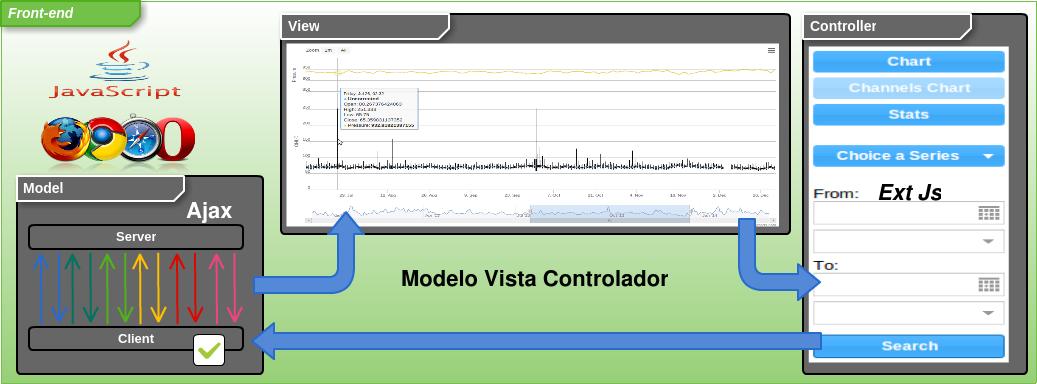
\includegraphics[keepaspectratio, width=1\textwidth]{./img/frontend.png}
	\caption{\emph{Front-end}. Patrón MVC.}   
	\label{fig:frontend}
\end{figure}
\section{Sencha ExtJs}
	El propósito de esta sección es explicar alguno de los aspectos básicos del framework. Empezaremos explicando como crear una aplicación básica
	basándonos en ExtJs. En la mayoría de los casos existe un solo documento HTML\cite{HTML} que contiene toda la aplicación. En este documento
	tenemos que cargar dos \emph{scripts} de la siguiente forma.
    		\begin{center} \texttt{<script type="text/javascript" src=\textquotedbl extjs/ext-all-debug.js\textquotedbl ></script>}  \end{center}
    		\begin{center} \texttt{<script type="text/javascript" src=\textquotedbl app.js\textquotedbl ></script>}  \end{center}
 	El primer \emph{script} contiene el framework que queremos utilizar. Es conveniente destacar que esta es una versión concebida para el proceso
	de desarrollo. Para la versión final es conveniente usar el \texttt{ext-all.js}.
 	\par
 	El segundo \emph{script} es el que contiene la lógica de nuestra aplicación. A continuación podemos ver el código mínimo para crear una
	aplicación. El código presentado será explicado a fondo.
	\begin{lstlisting}
Ext.application({
   name: 'HelloExt',
   launch: function() {
      Ext.create('Ext.container.Viewport', {
         layout: 'fit',
            items: [{
               title: 'Hello Ext',
               html : 'Hello! Welcome to Ext JS.'}] 
      }); 
   } 
});
	\end{lstlisting}
 	En la primera línea hacemos uso del singletone \texttt{Ext}. Este es un objeto que encapsula todas las clases, métodos y singletones
	proporcionados por el framework. La función utilizada \texttt{Ext.application} carga e inicializa una instancia de la clase
	\texttt{Ext.app.Application}. Esta clase representa una aplicación ExtJs single page. La llamada a esta función crea la variable global
	\texttt{MyApp}, que debe contener todas las clases e instancias de nuestra aplicación.
 	\par
 	En la segunda línea declaramos el nombre de nuestra aplicación. Seguidamente definimos la función \texttt{launch}. Esta es la función que debe
	lanzar  nuestra aplicación. La primera función invocada es \texttt{Ext.create} que crea una instancia de la clase proporcionada, en este caso
	\texttt{Ext.container.Viewport}. \texttt{Viewport} es un \emph{contenedor} que representa el área de aplicación y puede haber tan solo uno por
	aplicación. 
 	\par
 	La interfaz de usuario en una aplicación ExtJs es compuesta por \emph{componentes}. Un \emph{contenedor} es un \emph{componente} especial que
	contiene otros \emph{componentes}. En la figura \ref{fig:comps} podemos ver un ejemplo que ilustra esta jerarquía.
	\begin{figure}[h]
		\centering
		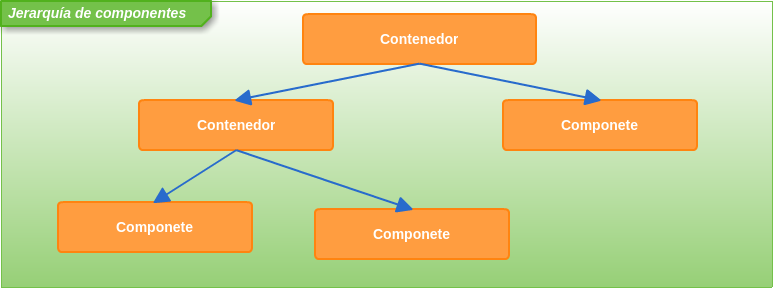
\includegraphics[keepaspectratio, width=1\textwidth]{./img/comps.png}
		\caption{Sencha ExtJs. Jerarquía de componentes.}   
		\label{fig:comps}
	\end{figure}
 	\par
 	El \texttt{Viewport} es el \emph{contenedor} que contiene todos los demás \emph{componentes} de nuestra aplicación. Los \emph{compenentes} de
	un \emph{contenedor} se especifican en el campo \texttt{items} que es una lista. En el ejemplo presentado tan solo tenemos un 
	\emph{conponente}, pero pueden ser añadidos más.
 	\par
 	Fijándonos en el código de ejemplo podemos ver que antes de definir el campo \texttt{items} definimos el campo \texttt{layout}. El \texttt{layout}
	especifica la forma en la que se posicionaran y ajustaran los \emph{componetes} hijos. En este caso el \texttt{layout} especificado es 
	\texttt{\cc fit\cc} en el que un solo hijo ocupa todo el espacio del padre. 
\section{Sencha ExtJs Component Manager}
	ExtJs ofrece el singletone \texttt{Ext.ComponentManager} que provee un registro con todos los componentes. Esto facilita la referencia a
	elementos desde cualquier punto del código. El propósito de esta sección es explicar como hacer uso de esta facilidad.
	\par
	Empezaremos especificando un requisito que  los componentes deben cumplir, estos deben definir un atributo \texttt{itemId}. Este atributo es
	el identificador del componente. El ámbito que tiene este identificador es local al contenedor que contiene el componente. Esto hace que los
	identificadores no tengan que ser únicos. 
	\par
	Es el singletone \texttt{Ext.ComponentQuery} el que nos permite realizar búsquedas de componentes en función del texttt{itemId}. Concretamente
	es \texttt{Ext.ComponentQuery.query()} el método que nos permite realizar las búsquedas. Este método acepta dos parámetros. El primer
	parámetro, \texttt{selector}, es un String y especifica el \texttt{itemId} que queremos buscar. El segundo parámetro, \texttt{root} es
	opcional y especifica el contenedor dentro de cual queremos hacer la búsqueda. Si el segundo parámetro es omitido la búsqueda se realizara
	entre todos los componentes. La función devuelve un array con todos los componentes que reúnen las condiciones, pudiendo ser este un array
	vacío. Eventualmente podemos hacer búsquedas más complejas, podemos buscar por tipo, atributos y mucho más. En este trabajo tan solo hemos
	utilizado queries simples, razón por la que no explicamos como se realizan estas queries avanzadas.
	\par
	La clase \texttt{Ext.container.Container} implementa las funciones \texttt{down()} y \texttt{query()}. Estas dos realizar una llamada a
	\texttt{Ext.ComponentQuery.query()} teniéndose a si mismo como parámetro \texttt{root}. Esto les permite hacer una búsqueda entre sus hijos.
	\par
	También existe el método \texttt{up()} implementado por \texttt{Ext.Component}. Este permite hacer una búsqueda similar a las anteriormente
	descritas. En este caso se navega hacia arriba en la jerarquía de componentes y se busca por componentes que reúnen los criterios. Esta
	función puede ser invocada sin ningún parámetro, caso en el que devuelve el padre inmediato del componente.
	\par
	Es conveniente también citar el parámetro \texttt{id} y la función \texttt{Ext.getCmp()}. Estos dos ofrecen una funcionalidad parecida a la
	anteriormente explicada, pero no deben ser usados con ese propósito. Estan considerados como obsoletos y pueden dar lugar a colisiones. 

\section{Sencha ExtJs Layouts}
	El propósito de esta sección es explicar los layouts utilizados en este trabajo. Tan solo explicaremos la funcionalidad de estos sin
	centrarnos en el uso que les hemos dado, este será explicado en las secciones venideras cuando proceda. En la figura \ref{fig:layouts} podemos
	ver una representación de los layouts que describiremos a continuación.
	\subsection{\texttt{Absolute}}
		Los \emph{componentes} hijo son posicionados mediante el uso de coordenadas \texttt{X,Y}. Las dimensiones de estos también se definen
		de forma estática mediante el uso de dos atributos, \texttt{height} and \texttt{width}. La posición y tamaño de los componentes se
		puede cambiar mediante el uso de las funciones \texttt{setPosition()} y \texttt{setSize()}.
	\subsection{\texttt{Accordion}}
		Este layout se asemeja a un acordeón. Los \emph{componentes} hijo pueden ser expandidos y colapsados, teniendo tan solo uno expandido
		a la vez. Los \emph{componentes} son ordenados en vertical ocupando todo el espacio disponible. Las funciones \texttt{expand} y
		\texttt{collapse} nos permiten expandir y colapsar los paneles hijo. También están presentes multitud de manejadores de eventos que
		podemos sobrescribir, en nuestro caso haremos uso del \texttt{beforeExpand} que se dispara antes de expandir un \emph{componente}. 
	\subsection{\texttt{Border}}
		Este layout nos permite tener hasta cinco \emph{componentes} dispuestos de la manera que podemos ver en la figura \ref{fig:layouts}.
		Los componentes hijos deben especificar al atribiuto \texttt{region} que determina el posicionamiento de estos. El campo puede tomar
		los siguientes valores \texttt{[north, east, south, west, center]}. No es necesario que estén presentes los cinco hijos, podemos
		omitir los no deseados. Esto hace que este layout sea muy flexible e interesante.
	\subsection{\texttt{Card}}
		Este layout maneja multiples \emph{componentes} hijo. Los hijos ocupan todo el espacio disponible, por lo que se solapan uno a otro.
		Esto hace que solo uno pueda ser visible a la vez. El layout asemeja una baraja de cartas donde solo una carta puede estar en la parte
		superior. La función que nos permite hacer visible un hijo es \texttt{setActiveItem()}. Esta función acepta el \emph{componente}, el
		\texttt{itemId} del \emph{componente} o el índice del \emph{componente}.
	\subsection{\texttt{Fit}}
		\texttt{Fit} es un layout muy simple, este tan solo acepta un hijo que ocupa todo el espacio que el padre ofrece. El \emph{componente}
		hijo se expandirá automáticamente para ajustarse al tamaño del padre.
	\subsection{\texttt{HBox y VBox}}
		Estos son dos layouts diferentes, pero muy parecidos, razón por la que serán explicados en la misma subsección. El \texttt{HBox}
		organiza sus elementos hijos de forma horizontal a lo largo del \emph{componente} padre. El \texttt{VBox} hace lo mismo, pero la
		organización es de forma vertical. Los componentes hijos pueden especificar el atributo \texttt{flex}, este atributo determina como
		será repartido el espacio disponible entre los diferentes hijos. Para ilustrar el funcionamiento del \texttt{flex} expondremos un
		ejemplo. Teniendo dos \emph{componentes} hijo con \texttt{1} y \texttt{2} de \texttt{flex} respectivamente, el primero ocupara 1/3 y el
		segundo 2/3 del espacio total.
	\begin{figure}[h]
		\centering
		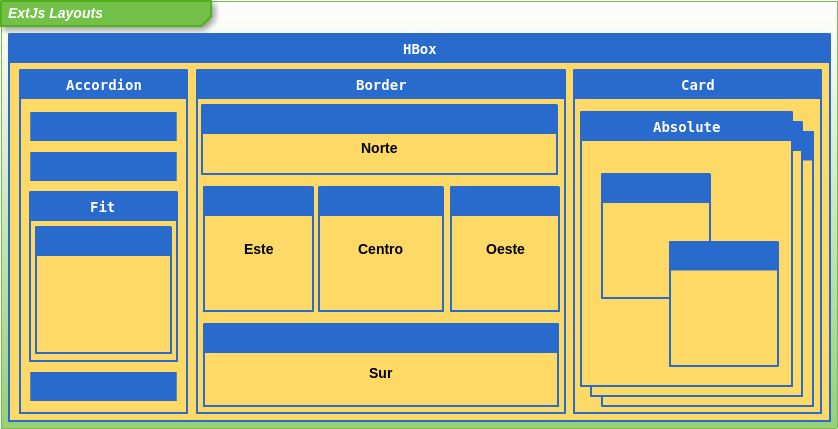
\includegraphics[keepaspectratio, width=1\textwidth]{./img/layouts.png}
		\caption{Sencha ExtJs. Layouts.}   
		\label{fig:layouts}
	\end{figure}

\section{Sencha ExtJs Lazy instantiation}
	La inicialización perezosa es una técnica que consiste en retrasar la creación de recursos hasta el momento en el que sean necesarios. Como
	hemos visto en la sección dedicada a los layouts en muchos casos los componentes no son visibles. Tener que crear todos los componentes al
	inicializar la aplicación no es muy eficiente, dado que tan solo unos pocos son visibles. Crear tan solo los componentes visibles y después ir
	creando los componentes según se vayan necesitando supone un incremento en el rendimiento. En páginas pequeñas con pocos componentes el
	aumento no es apreciable, sin embargo en páginas que manejan multitud de componentes el incremento puede ser drástico. 
	\par
	Para implementar esta inicialización perezosa ExtJs se basa en la jerarquía de componentes previamente explicada. Cuando un componente es
	creado también se crean todos los componentes hijos que deben ser visibles en ese momento. Tal y como explicamos los componentes hijos se
	definen en el campo \texttt{items}. A continuación podemos ver un pequeño ejemplo. 
	\begin{lstlisting}
items:[
   Ext.create('Ext.form.field.Text',{
      fieldLabel:'Foo'}),
   Ext.create('Ext.form.field.Text', {
      fieldLabel: 'Bar'})]
	\end{lstlisting}
	El ejemplo presentado anteriormente no habilita la inicialización perezosa. Para este propósito tenemos que evitar el uso de la función
	\texttt{Ext.create()}. Tenemos que especificar los componentes hijos como objetos de configuración. A continuación se presenta un ejemplo.
	\begin{lstlisting}
items: [{
   xtype: 'textfield',
   fieldLabel: 'Foo'},
{
   xtype: 'textfield',
   fieldLabel: 'Bar'}]
	\end{lstlisting}
	La diferencia que podemos apreciar entre los dos ejemplos es el atributo \texttt{xtype}. Este especifica la clase que tendrá el componente.
	Como podemos ver no se especifica el nombre completo de la clase. \texttt{xtype} acepta una serie atajos para referenciar a las clases. En
	nuestro caso la clase \texttt{Ext.form.field.Text} es referenciada por el \texttt{xtype:\cc textfield\cc}.
	\par
	La lista completa de \texttt{xtypes} aceptados podemos ver en la documentación de ExtJs\cite{ExtJsDoc}. Eventualmente podemos extender esta
	lista declarando nuestros propios \texttt{xtypes}. Esto se hace especificando el campo \texttt{xtype} a la hora de definir nuestra clase. A
	continuación presentamos un pequeño ejemplo.
	\begin{lstlisting}
Ext.define('MyApp.PressMeButton', {
   extend: 'Ext.button.Button',
   xtype: 'pressmebutton',
   text: 'Press Me'});
	\end{lstlisting}

\section{Sencha ExtJs Events}
	Las clases y componentes de ExtJs disparan multitud de eventos a lo largo de su ciclo de vida. Los eventos se disparan cuando algo interesante
	le ocurre a nuestro componente. Un ejemplo es el evento \texttt{afterrender} que se dispara después de mostrar en pantalla el componente.
	\par
	La parte interesante de los eventos es que podemos definir funciones, \texttt{listeners}, que se ejecuten cuando se produzca un evento
	determinado. De esta manera somos capaces de responder a dichos eventos. A continuación presentamos un ejemplo en el que podemos ver como
	manejar dichos eventos. En el ejemplo trataremos el evento \texttt{click}, evento que se dispara al hacer \emph{click} sobre un componente. 
	\begin{lstlisting}
Ext.create('Ext.Button',{
   text: 'Click Me',
   renderTo: Ext.getBody(),
   listeners:{
      click: function(){
         Ext.Msg.alert('I was clicked!');}
   }
});
	\end{lstlisting}
	\par
	ExtJs también nos permite configurar eventos propios. Estos eventos se declaran como si fuesen eventos normales. La peculiaridad esta en que
	somos nosotros los que tenemos que disparar esos eventos. Para disparar un evento tenemos que hacer uso de la función \texttt{fireEvent} que
	acepta como parámetros el evento que queremos disparar y todos los parámetros que la función encargada del evento necesite. A continuación
	podemos ver un pequeño ejemplo de como declarar y disparar un evento propio, que tiene como nombre \texttt{myEvent}.
	\begin{lstlisting}
var button = Ext.create('Ext.Button',{
   text: 'Custom Event',
   renderTo: Ext.getBody(),
   listeners:{
      myEvent: function(number){
         Ext.Msg.alert('Custom event fired, number: '+number);}
   }
});

button.fireEvent('myEvent', 42);
	\end{lstlisting}

\section{ExtJs History stack}
	La aplicación Web que estamos desarrollando es una aplicación \emph{single page}. Este modelo rompe con el patrón tradicional de navegación
	por el historial usando los botones \emph{Forward/Back}. Esto presenta un problema de usabilidad cuando el usuario utiliza el botón de
	navegación hacia atrás, este espera volver al estado anterior de la aplicación, sin embargo sera cargada la página anterior del historial y
	nuestra aplicación \emph{single page} será descargada.
	\par
	La solución que la mayoría de aplicaciones \emph{single page} han adoptado se basa en el \emph{Fragment Identifier}  o \emph{hash}, nombre que
	recibe porque va precedido del símbolo \textbf{\#}. El \emph{hash} es una parte opcional de la URL que históricamente se utilizaba para navegar
	por documentos largos, un cambio en el \emph{hash} hace que se muestres diferentes partes del documento.
	\par
	Actualmente el \emph{hash} es usado por aplicaciones \emph{single page} para manipular la pila de historial. El hash es cambiado acuerdo al
	estado de la aplicación. Esto hace que los cambios en la aplicación sean registrados en la pila de historial.
	\par
	Al pulsar el botón de navegación hacia atrás el \emph{hash} de la URL cambia a su estado anterior. Nuestra aplicación debe ser capaz de
	detectar los cambios en el \emph{hash} y actual acuerdo a estos. De esta manera podemos preservar la funcionalidad de los botones de
	navegación \emph{Forward/Back}. 
	\par
	Para implementar la funcionalidad anteriormente descrita ExtJs nos ofrece el singletone \texttt{Ext.util.History}. Para inicializar este módulo
	tenemos que invocar la función \texttt{Ext.History.init()}. Una vez inicializado este módulo podemos hacer cambios en el \emph{hash} invocando
	la función \texttt{Ext.History.add()}. Esta función acepta como parámetro el valor del \emph{hash}. 
	\par
	Para detectar y actual acorde a los cambios del \emph{hash} tenemos que inicializar un \texttt{listener}. El evento que vamos a capturar es
	\texttt{change}. A continuación podemos ver un pequeño código de como inicializar el \texttt{listener}.
	\begin{lstlisting}
Ext.History.on('change', function(hash){
   switch(hash){
      case: 'Foo':
         //Actuar acuerdo al hash Foo
         break;
      case: 'Bar'
         //Actuar acuerdo al hash Bar
         break;
   };
});
	\end{lstlisting}
	\par
	El propósito de esta sección ha sido explicar el problema que surge con el historial de navegación y como prevenir lo haciendo uso del
	\texttt{Ext.History}. Del uso concreto que hemos hecho de este módulo hablaremos en secciones futuras de este capítulo.

\section{\emph{Modelo}}
	El \emph{modelo} es el encargado de manejar los datos de una aplicación. En el caso del \emph{front-end} los datos de la aplicación deben ser
	servidos por el \emph{back-end}. El \emph{modelo} es el encargado de realizar la comunicación con el \emph{back-end}. 
	\par
	Tal y como especificamos en el  capítulo anterior el protocolo para la comunicación entre los dos módulos es \emph{HTTP}. Nuestro
	\emph{front-end} es el que empieza la comunicación enviando un mensaje de petición y el \emph{back-end} responde a esa peticion con un mensaje
	de respuesta. El \emph{modelo} es el encargado de construir y enviar los mensajes de petición y después interpretar los mensajes de respuesta.
	\par
	Para dotar el \emph{modelo} de la funcionalidad necesaria vamos a ayudarnos de las facilidades que nos ofrece ExtJs, concretamente vamos a
	utilizar el singletone \texttt{Ext.Ajax}. Ajax\cite{AjaxWiki} es una técnica de desarrollo Web donde cliente y servidor mantienen una
	comunicación asíncrona en segundo plano. \texttt{Ext.Ajax} es un singletone de la clase \texttt{Ext.data.Connection}, clase que encapsula la
	lógica necesaria para realizar una comunicación Ajax. 
	\par
	Concretamente vamos a hacer uso de la función \texttt{Ext.data.Connection.request}. Esta función envía una petición \emph{HTTP} a un servidor
	remoto. La función acepta un solo parámetro que es un objeto cuyas propiedades definen el comportamiento de la función. Las propiedades de las
	que nosotros haremos uso están detalladas a continuación. 
	\begin{itemize}
  		\item	\texttt{url}. 	La URL a la que enviaremos la petición. En nuestro caso \emph{back-end} y \emph{front-end} estarán albergados en
		  	el mismo \emph{host}. Esto nos permite no especificar el \emph{host}, la petición se hará al \emph{host} utilizado para cargar
			la aplicación. En la URL tan solo tendremos que especificar el servicio deseado y los parámetros que acompañan a este.
			Seguidamente presentamos un ejemplo del valor que puede tomar el campo \texttt{url}.
    				\begin{center} \texttt{url: \cc/nmdadb/cannel/stats/default/default\cc}  \end{center}
		\item	\texttt{method}. El método que especifica nuestro mensaje de petición. Los mensajes \emph{HTTP} de petición pueden especificar
		  	un método. Si este campo es dejado vacío el método utilizado será \texttt{GET}. La mayoría de los servicios ofrecidos por el
			\emph{back-end} aceptan un método \texttt{GET}, pero el servicio \texttt{nmdbMarkNull} acepta un método \texttt{POST}.
		\item	\texttt{success}. La función a ser llamada al completar exitosamente la petición. Esta función a su vez acepta como parámetro
		  	\texttt{response}. Este parámetro contiene los datos del mensaje de respuesta.
		\item	\texttt{failure}. La función a ser llamada al completar sin éxito la petición. Esta función también acepta el parámetro
		  	\texttt{response} que podemos utilizar para identificar la causa del fallo.
		\item	\texttt{timeout}. El numero de milisegundos en los que el \emph{back-end} debe responder. Si el tiempo expira la solicitud se
		  	considera como fallida. 
	\end{itemize}
	Más allá de \emph{Ext.data.Connection} el framework ofrece abstracciones de un nivel superior. La clase \emph{Ext.data.Model} es una
	representación de un objeto utilizado por nuestra aplicación. Estos modelos son usados por la clase \emph{Ext.data.Store}, que encapsula
	instancias de un modelo. La clase \emph{Ext.data.Store} también hace uso del \emph{Ext.data.proxy.Proxy}, abstracción que permite cargar y
	guardad datos de un modelo. 
	\par
	Estas abstracciones son muy útiles, pero algo complejas. Al no estar acostumbrado a trabajar con ellas el autor de este trabajo ha preferido
	utilizarlas lo menos posible. Por esta razón la mayoría de los datos se manejan usando el \texttt{Ext.data.Connection}, hemos utilizado el
	\texttt{Ext.data.Store} en casos muy específicos.
